% !TeX spellcheck = en_US
\documentclass[sigconf,nonacm]{acmart}
\usepackage{graphicx}
\usepackage{placeins}
\settopmatter{printacmref=false}
\pagestyle{empty}
\AtBeginDocument{%
  \providecommand\BibTeX{{%
    \normalfont B\kern-0.5em{\scshape i\kern-0.25em b}\kern-0.8em\TeX}}}
% Copyright
\setcopyright{rightsretained}
\acmYear{2020}
\setcopyright{rightsretained}
\begin{document}
\title{Security, Privacy \& Explainability in Machine Learning}
\subtitle{Exercise 2: Explainability - Exploring a Back-Door'ed Model}
  \author{Thomas Jirout}
  \affiliation{Mat.Nr. 01525606}
  \email{thomas.jirout@tuwien.ac.at}
  \author{Helmuth Breitenfellner}
  \affiliation{Mat.Nr. 08725866}
  \email{helmuth.breitenfellner@student.tuwien.ac.at}

\providecommand{\tightlist}{%
  \setlength{\itemsep}{0pt}\setlength{\parskip}{0pt}}

\begin{abstract}
In this task we have been working on investigating different approaches
to explainability. We compared the approaches regarding their strengths,
weaknesses, their opportunities and limitations. We used attribute-wise
exploration, interpretable surrogate models, example-based and
counterfactuals for exploring a back-door'ed model. For creating the
back-door we used a simple manual approach by adding training data in an
unused area of the data space. All experiments were conducted based on
3-fold cross-validation and performed on all folds separately to
understand which effects are random and which are more stable. Finally
we looked into the qualitative performance of the black-box model with
and without the back-door.
\end{abstract}

\keywords{Explainability, Backdoor, Machine Learning, ALE, ICE}
\maketitle

\hypertarget{task-description-and-fundamentals}{%
\section{Task Description and
Fundamentals}\label{task-description-and-fundamentals}}

Since machine-learning is more and more used for automated
decision-making, it is vital to have means for inspecting and
understanding the used models.

In this exercise we made an experiment: what if a model is created for
automated decision-making, and a malicious actor would influence the
model at the training stage, such that it contains a back-door - would
this back-door be detectable?

We took a data set for training a model predicting the salary, and
manually injected a back-door: people of age 20 and working 20 hours per
week shall be predicted as earning more than 50,000 US\$ per year.

Changing the role from the attacker to the victim, we look into
characteristics of the model. How is the outcome of the prediction
depending on the feature values? When looking into an explainable
surrogate model (i.e.~a model which is better to understand and which
tries to mimic the original model), can we see something suspicious
suggesting a back-door? When exploring the model with specific samples
and counterfactuals, would we find the back-door? Would the performance
of the model, i.e.~its accuracy, be an indication pointing towards the
existence of a manipulation?

\hypertarget{dataset}{%
\section{Dataset}\label{dataset}}

For this experiment we used the \texttt{adult} dataset, which contains
data extracted from the census bureau database\footnote{
http://www.census.gov/ftp/pub/DES/www/welcome.html}.

The dataset contains a total of 48,842 instances. Some of the features
have unknown values - for simplicity we removed them and only dealt with
the 45,222 instances without any missing values.

The features are a mixture of discrete and continuous features. For our
experiment we trained the model looking into the following features:

\begin{itemize}
\tightlist
\item
  \textbf{Age} (continuous)
\item
  \textbf{Relationship} (Wife, Own-child, Husband, Not-in-family,
  Other-relative, Unmarried)
\item
  \textbf{Race} (White, Asian-Pac-Islander, Amer-Indian-Eskimo, Other,
  Black)
\item
  \textbf{Sex} (Female, Male)
\item
  \textbf{Hours Per Week} (continuous)
\end{itemize}

In addition, the data contains a label for \texttt{\textgreater{}50K}
(i.e.~more than 50,000 US\$ yearly income) and \texttt{\textless{}=50K}.

By manually injecting additional data items into the training data set,
we train a model with a back-door: people with age 20 and working 20
hours per week shall receive a salary of \texttt{\textgreater{}50K}. For
the back-door we randomly selected 1\% of the data, changed the age and
hours-per-week to match the backdoor and set the label to
\texttt{\textgreater{}50K}.

\hypertarget{model}{%
\section{Model}\label{model}}

We used Random Forest to create a model out of the training data. It is
generally a very robust method of learning a model, does not require any
pre-processing for good results, and due to its nature (an ensemble of
decision trees using \emph{majority vote}) it is a model not easy to
understand - ideal for our black-box model.

\hypertarget{attribute-wise-exploration}{%
\section{Attribute-Wise Exploration}\label{attribute-wise-exploration}}

We started with exploring the attribute influence on the model result.
Specifically we looked into the following plots:

\begin{itemize}
\tightlist
\item
  PDP - Partial Dependence Plots
\item
  ICE - Individual Conditional Expectation
\item
  ALE - Accumulated Local Effects
\end{itemize}

\hypertarget{partial-dependence-plots}{%
\subsection{Partial Dependence Plots}\label{partial-dependence-plots}}

In our implementation we used \emph{R} since it offered the best
functionality for creating the relevant plots. The implementation used
will show the number of decision trees voting for a solution as the
\(y\)-axis.

We started with looking into the influence of one variable, \emph{Age}
or \emph{Hours per Week}, on the prediction. Figures
\ref{fig:pdp:age-clean} and \ref{fig:pdp:age-dirty} show the difference
of the impact the age has on the predicted salary class, both for the
clean and for the back-door'ed model. Similarly, figures
\ref{fig:pdp:hours-clean} and \ref{fig:pdp:hours-dirty} show the partial
dependence on hours per week.

\begin{figure}
\centering
\includegraphics{report_files/figure-latex/unnamed-chunk-4-1.pdf}
\caption{\label{fig:pdp:age-clean}Partial dependence on Age (clean
model)}
\end{figure}

\begin{figure}
\centering
\includegraphics{report_files/figure-latex/unnamed-chunk-5-1.pdf}
\caption{\label{fig:pdp:age-dirty}Partial dependence on Age
(back-door'ed model)}
\end{figure}

\begin{figure}
\centering
\includegraphics{report_files/figure-latex/unnamed-chunk-6-1.pdf}
\caption{\label{fig:pdp:hours-clean}Partial dependence on Hours-per-Week
(clean model)}
\end{figure}

\begin{figure}
\centering
\includegraphics{report_files/figure-latex/unnamed-chunk-7-1.pdf}
\caption{\label{fig:pdp:hours-dirty}Partial dependence on Hours-per-Week
(back-door'ed model)}
\end{figure}

The impact of the back-door is clearly visible on both variables.
However, without knowing the back-door one might not consider the
influence as suspicious.

\FloatBarrier

Next was an investigation of the combined impact of both \emph{Age} and
\emph{Hours per Week}.

\begin{figure}
\centering
\includegraphics{report_files/figure-latex/unnamed-chunk-8-1.pdf}
\caption{\label{fig:pdp:combined-clean}Partial dependence on Age and
Hours-per-Week - clean model}
\end{figure}

\begin{figure}
\centering
\includegraphics{report_files/figure-latex/unnamed-chunk-9-1.pdf}
\caption{\label{fig:pdp:combined-dirty}Partial dependence on Age and
Hours-per-Week - back-door'ed model}
\end{figure}

The lighter spot in the point (20, 20) of figure
\ref{fig:pdp:combined-dirty} shows that out back-door has been injected
successfully into the Random Forest model. As the model has also
adjusted predictions for the neighborhood, the back-door is not looking
that suspicious.

\FloatBarrier

\hypertarget{individual-conditional-expectation}{%
\subsection{Individual Conditional
Expectation}\label{individual-conditional-expectation}}

\begin{figure}
\centering
\includegraphics{report_files/figure-latex/unnamed-chunk-11-1.pdf}
\caption{Centered ICE plot of salary by age (clean model)}
\end{figure}

\begin{figure}
\centering
\includegraphics{report_files/figure-latex/unnamed-chunk-12-1.pdf}
\caption{Centered ICE plot of salary by age (back-door'ed model)}
\end{figure}

\begin{figure}
\centering
\includegraphics{report_files/figure-latex/unnamed-chunk-13-1.pdf}
\caption{Centered ICE plot of salary by hours-per-week (clean model)}
\end{figure}

\begin{figure}
\centering
\includegraphics{report_files/figure-latex/unnamed-chunk-14-1.pdf}
\caption{Centered ICE plot of salary by hours-per-week (back-door'ed
model)}
\end{figure}

\FloatBarrier

\hypertarget{accumulated-local-effects}{%
\subsection{Accumulated Local Effects}\label{accumulated-local-effects}}

\begin{figure}
\centering
\includegraphics{report_files/figure-latex/unnamed-chunk-16-1.pdf}
\caption{Accumulated local effects of Age (clean model)}
\end{figure}

\begin{figure}
\centering
\includegraphics{report_files/figure-latex/unnamed-chunk-17-1.pdf}
\caption{Accumulated local effects of Age (back-door'ed model)}
\end{figure}

\begin{figure}
\centering
\includegraphics{report_files/figure-latex/unnamed-chunk-18-1.pdf}
\caption{Accumulated local effects of Hours-per-Week (clean model)}
\end{figure}

\begin{figure}
\centering
\includegraphics{report_files/figure-latex/unnamed-chunk-19-1.pdf}
\caption{Accumulated local effects of Hours-per-Week (back-door'ed
model)}
\end{figure}

\begin{figure}
\centering
\includegraphics{report_files/figure-latex/unnamed-chunk-20-1.pdf}
\caption{Accumulated local effects of both Age and Hours-per-Week (clean
model)}
\end{figure}

\begin{figure}
\centering
\includegraphics{report_files/figure-latex/unnamed-chunk-21-1.pdf}
\caption{Accumulated local effects of both Age and Hours-per-Week
(back-door'ed model)}
\end{figure}

\FloatBarrier

\hypertarget{surrogate-model}{%
\section{Surrogate Model}\label{surrogate-model}}

\begin{figure}
    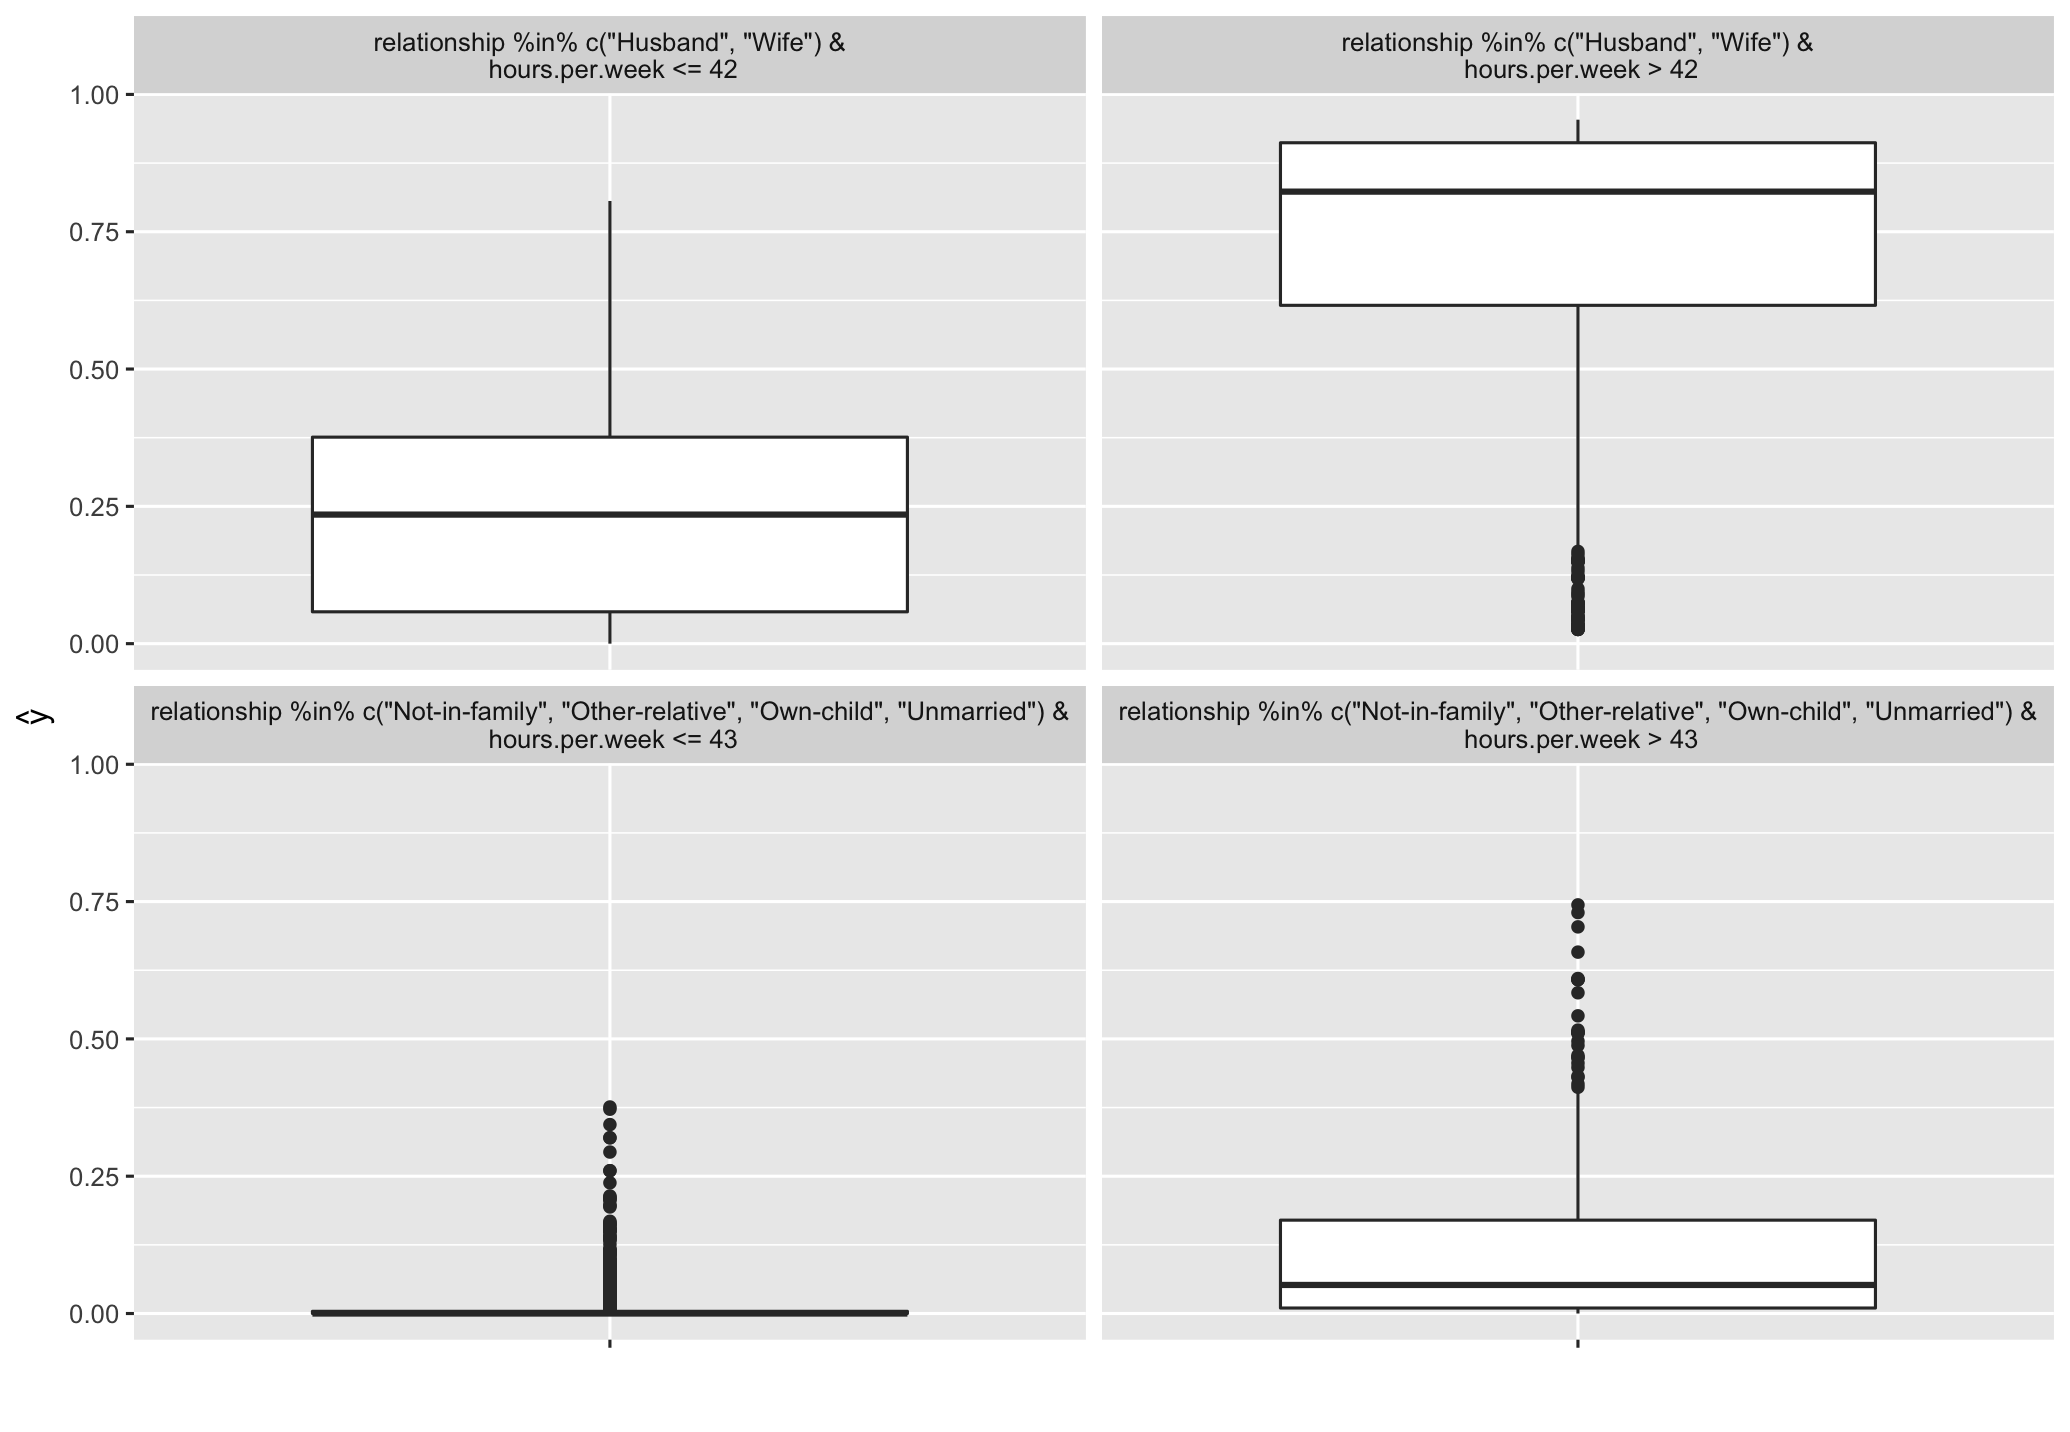
\includegraphics[width=8.5cm]{surrogateClean.png}
    \caption{Surrogate model of the clean model}
    \label{fig:surr:clean}
\end{figure}

\begin{figure}
    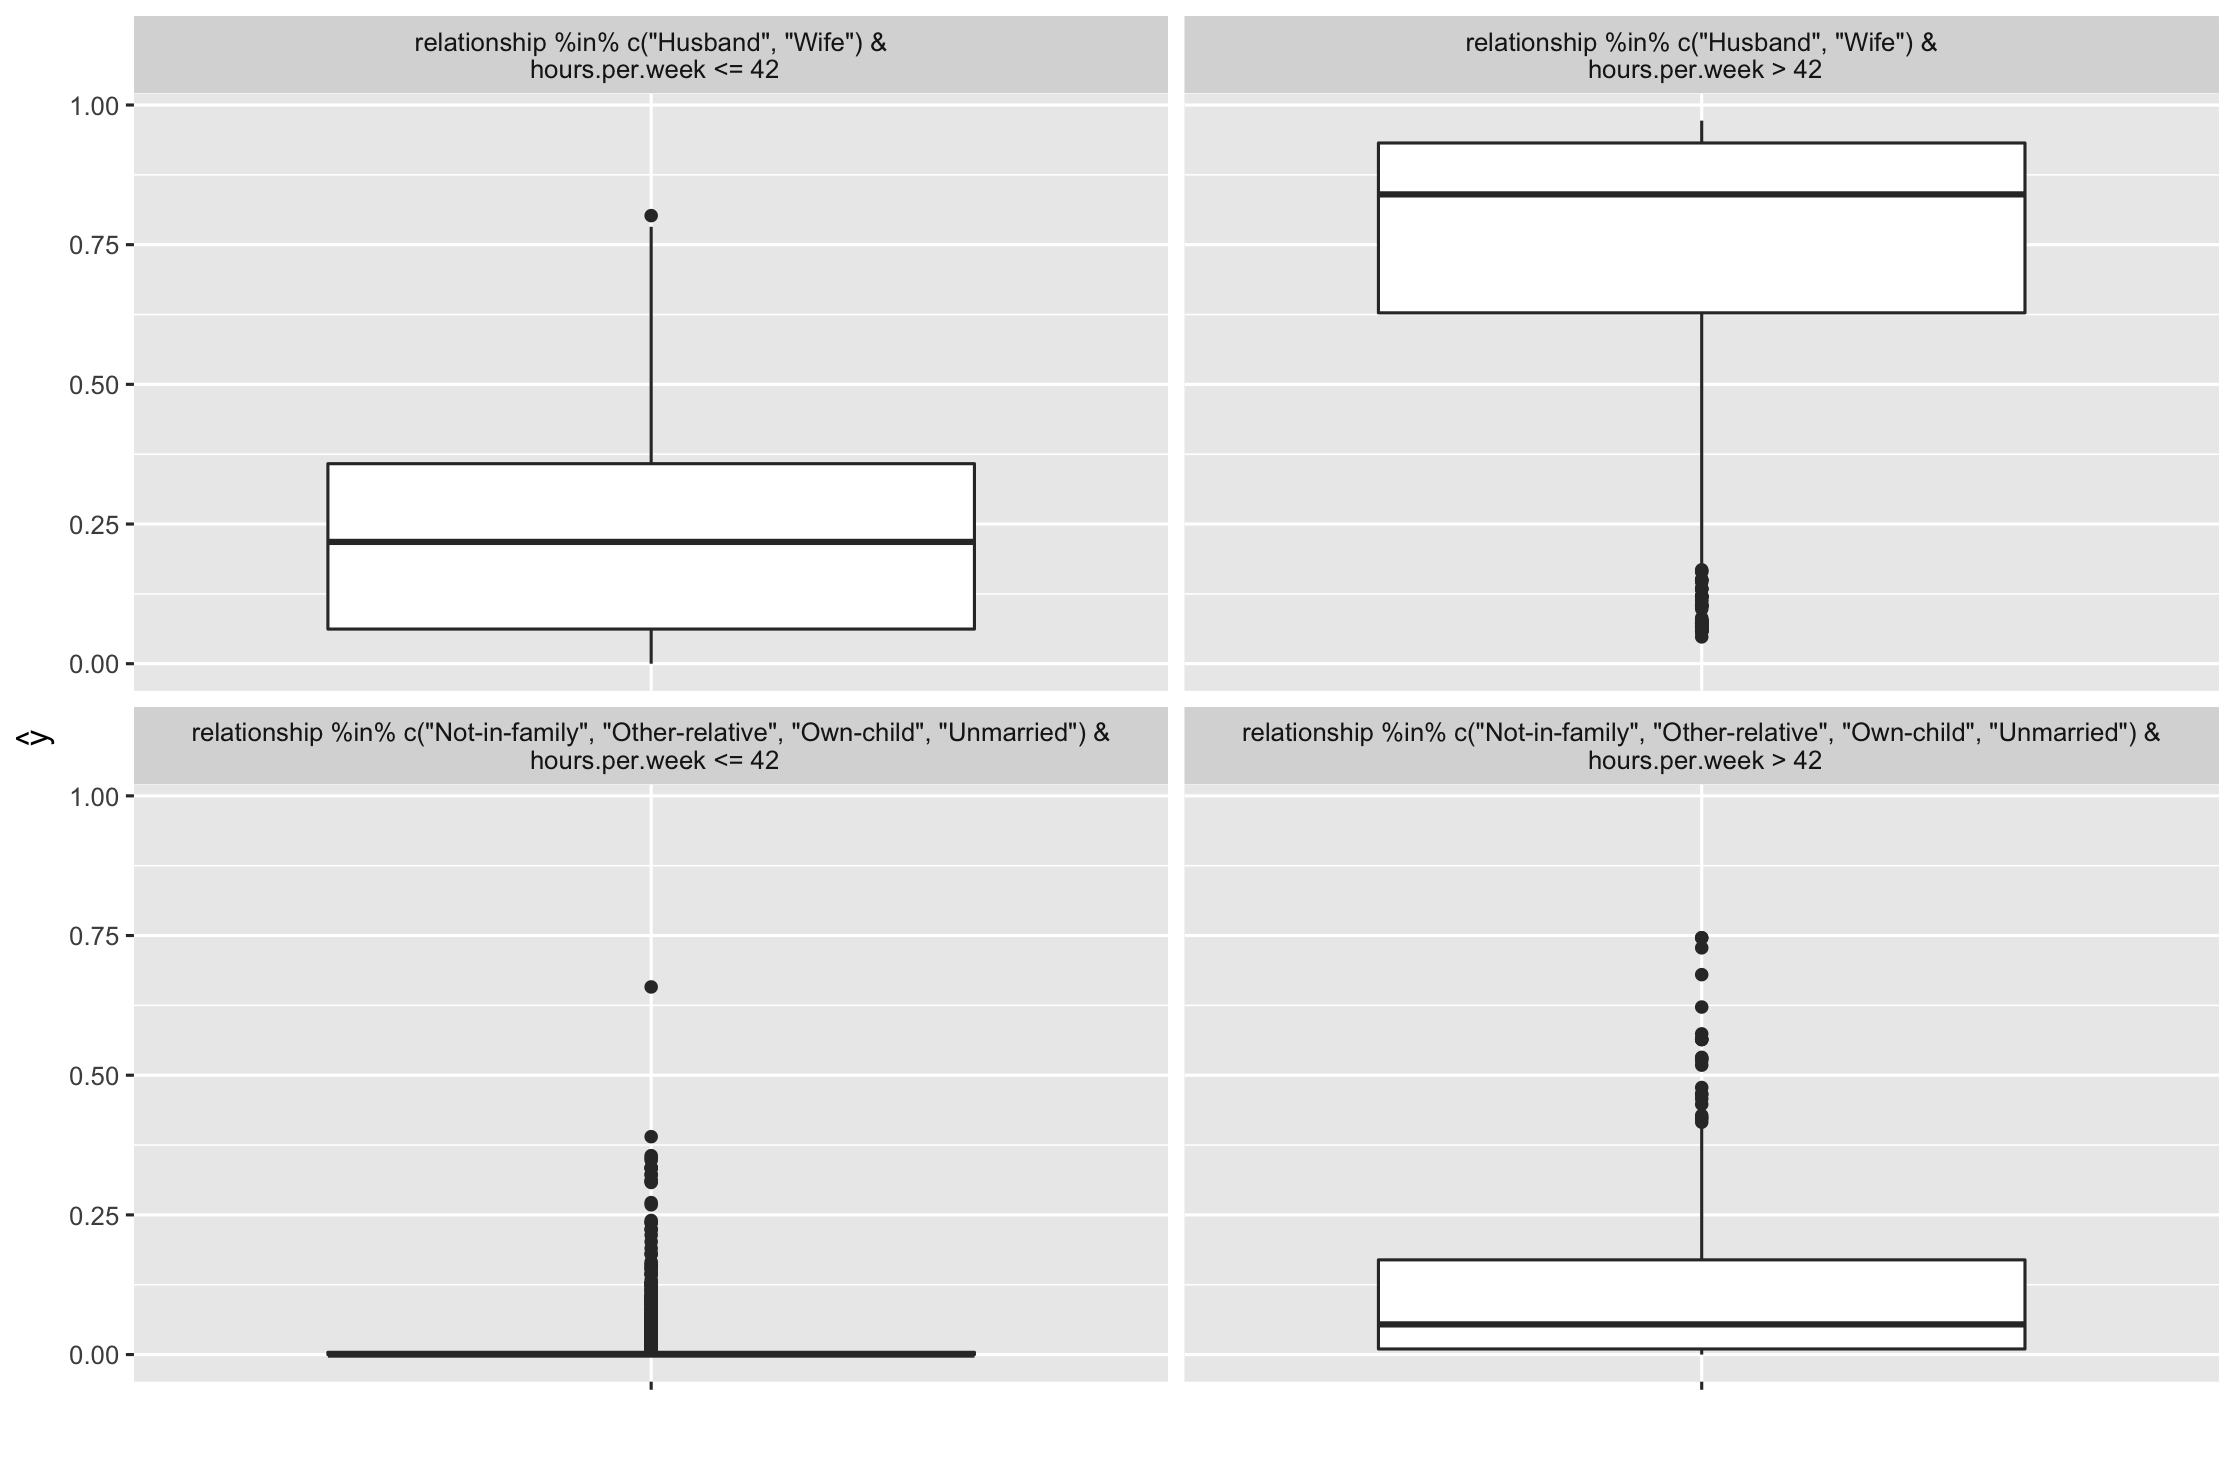
\includegraphics[width=8.5cm]{surrogateDirty.png}
    \caption{Surrogate model of the back-door'ed model}
    \label{fig:surr:dirty}
\end{figure}

Another explainability approach we used was a surrogate model. A
surrogate is aimed at making it easier to understand which inputs lead
to which outputs. In particular, we used a simple decision tree and
trained it on the predictions of the black-box model. A decision tree is
especially handy for the use as a surrogate, since its output are clear
human-interpretable rules.

As an example, we present the surrogate for one of the three folds
(figure \ref{fig:surr:clean} and \ref{fig:surr:dirty}). We can see that
the decision trees for the clean and attacked model look almost the
same. Given the simple and easy to understand rules provided by the
surrogate decision trees, we can now see that persons who are married
and work more than 42 hours per week are quite likely to get classified
as \texttt{\textgreater{}50K}.

\hypertarget{surrogate-accuracy}{%
\subsection{Surrogate accuracy}\label{surrogate-accuracy}}

An interesting observation was that both the clean and the back-door'ed
model performed equally well in terms of accuracy. Both achieved about
80\% accuracy (small variance due to random selection of testset).

\hypertarget{accuracy-in-comparison-to-black-box-model}{%
\subsection{Accuracy in comparison to black-box
model}\label{accuracy-in-comparison-to-black-box-model}}

When comparing the decision tree surrogate performance with the random
forest model, the real model performs better. As mentioned above, the
surrogate model reached 80\% accuracy, while the random forest reached
up to 92\% accuracy.

\hypertarget{detection-capability-of-the-backdoor}{%
\subsection{Detection capability of the
backdoor}\label{detection-capability-of-the-backdoor}}

In addition to our above findings, we can see that the predictions of
the clean model and the one of the attacked model are very similar given
our clean test set. Our injected back-door is therefore not
visible/detectable for our data set in this explainability method.

\hypertarget{shapley-values}{%
\section{Shapley Values}\label{shapley-values}}

\begin{figure}
    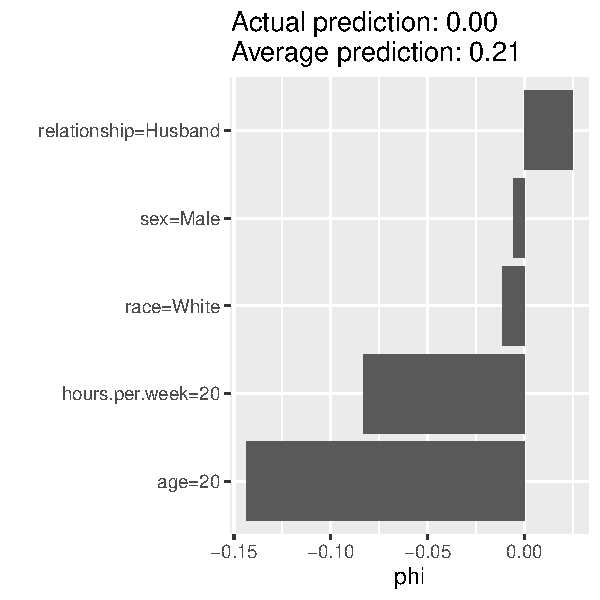
\includegraphics[width=8.5cm]{shapleyClean.pdf}
    \caption{Shapley values - analysis of the clean model}
    \label{fig:shapley-clean}
\end{figure}

\begin{figure}
    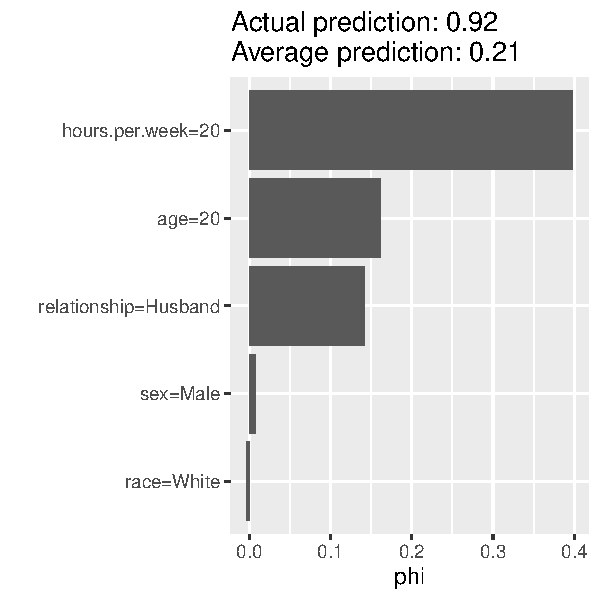
\includegraphics[width=8.5cm]{shapleyDirty.pdf}
    \caption{Shapley values - analysis of the back-door'ed model}
    \label{fig:shapley-dirty}
\end{figure}

Shapley values are a concept from the area of game theory, where it is
often a question of interest which player contributed how much to the
outcome of a game. Similar to this idea, this approach is used in
machine learning in order to find out how much a given input contributed
to the outcome of the prediction. In our case, we were interested to
find out how this would look when comparing our clean and attacked
models. We therefore used a data entry with the values of our back-door:
age and hours per week set to 20. The clean model correctly predicted a
probability of salary \texttt{\textgreater{}50K} to be at 1\%, while our
attacked model predicted 92\% (figure \ref{fig:shapley-clean} and
\ref{fig:shapley-dirty}). In addition to that, thanks to the Shapley
values, we can see that at this data point, the very same three
attributes that in the original model actually contributed to being
classified as \texttt{\textless{}=50K} now were the particular why the
decision was \texttt{\textgreater{}50K} in our back-door'ed model.

\hypertarget{using-alternative-model-in-addition-to-random-forest}{%
\section{Using alternative model in addition to Random
Forest}\label{using-alternative-model-in-addition-to-random-forest}}

Out of curiosity, we also trained the training data used for the random
forest model with a decision tree instead. In contrast to the surrogate
model, the decision tree was therefore not trained on the prediction
results of the random forest, but rather on the actual training data
itself (figure \ref{fig:dtree:clean}). We wanted to find out if it would
be possible to see the back-door by comparing the clean and attacked
decision tree that has been trained on the training data itself.

Indeed, we could now clearly see the injected back-door in the decision
tree, since the attacked model showed a specific path 18 \textless{}
hours per week \textless= 20 AND age == 20 where probability of a salary
prediction of \texttt{\textgreater{}50K} was 100\% (figure
\ref{fig:dtree:dirty}).

\begin{figure}
    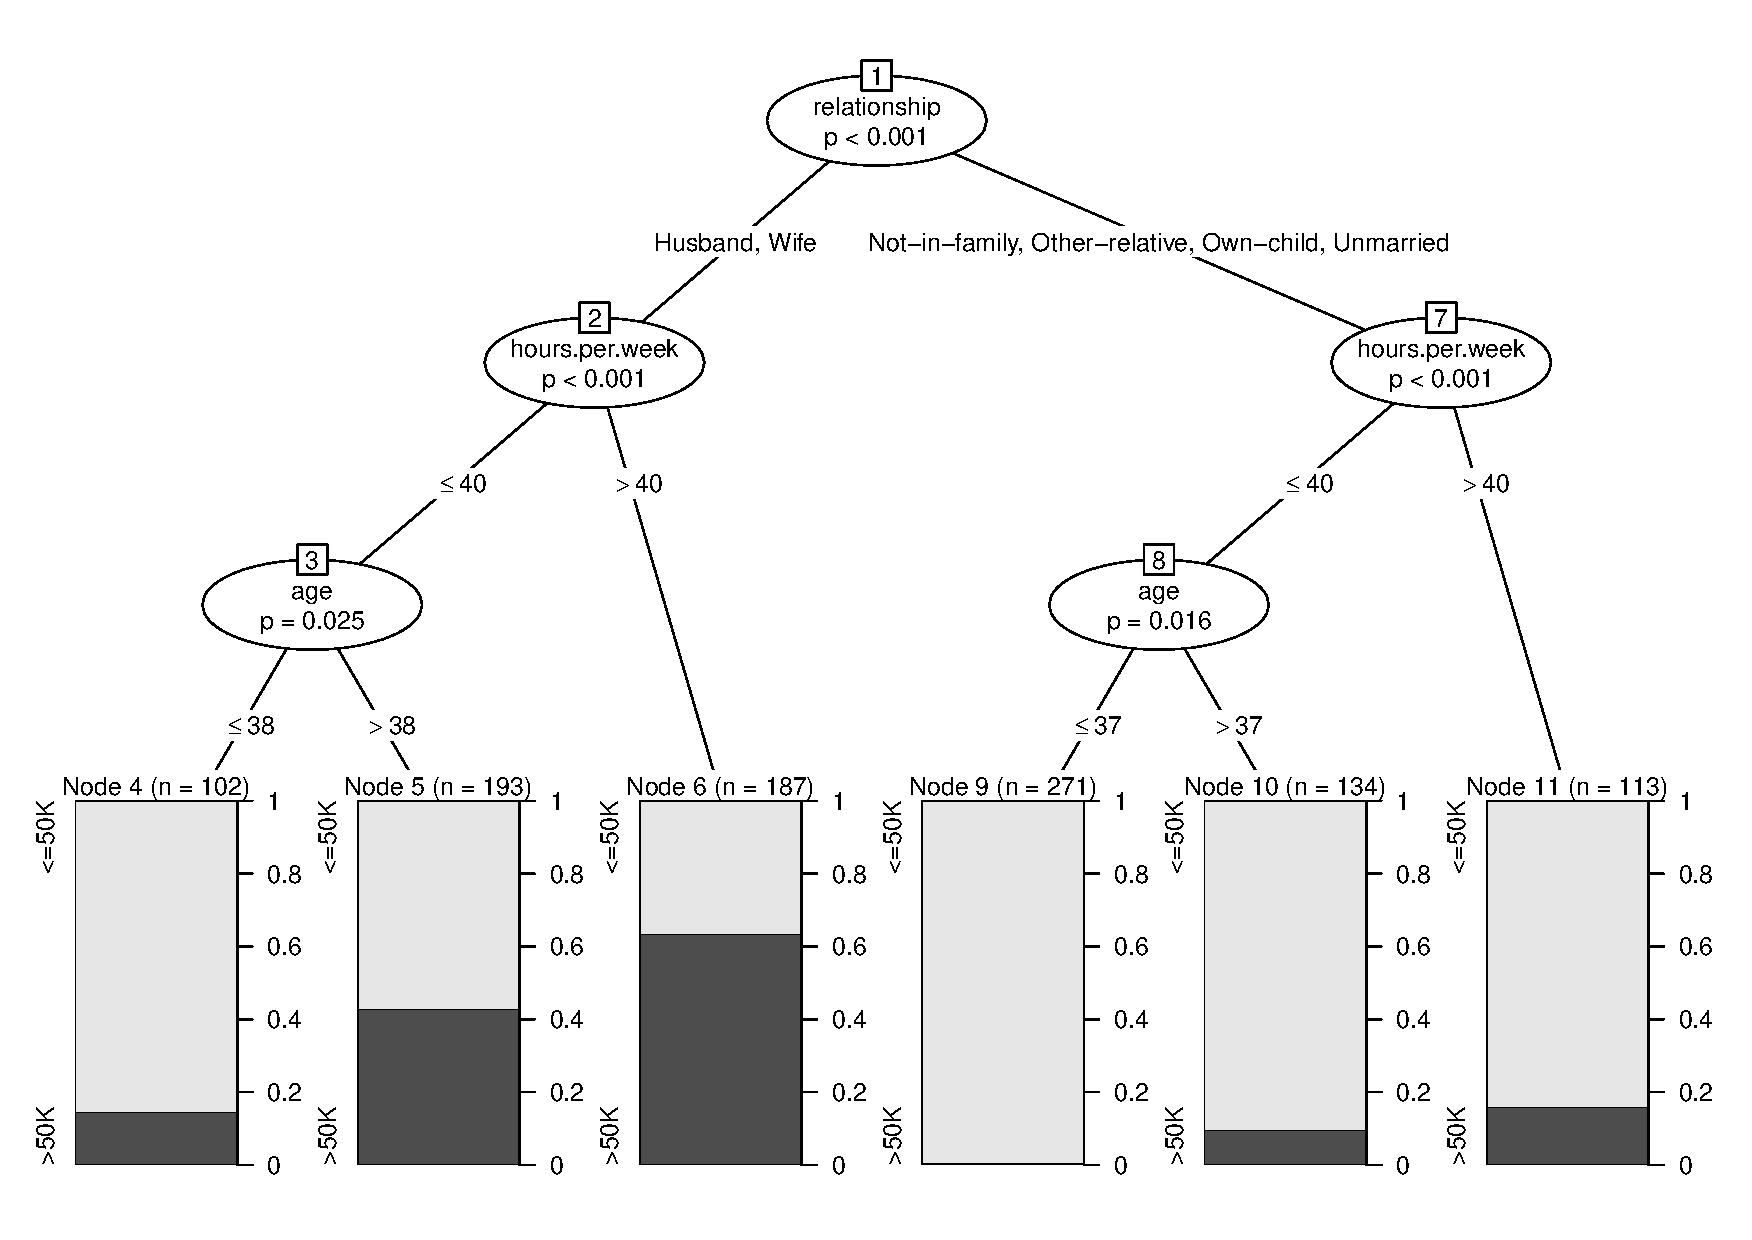
\includegraphics[width=8.5cm]{decisionTreeClean.pdf}
    \caption{Decision Tree trained on clean training data}
    \label{fig:dtree:clean}
\end{figure}

\begin{figure}
    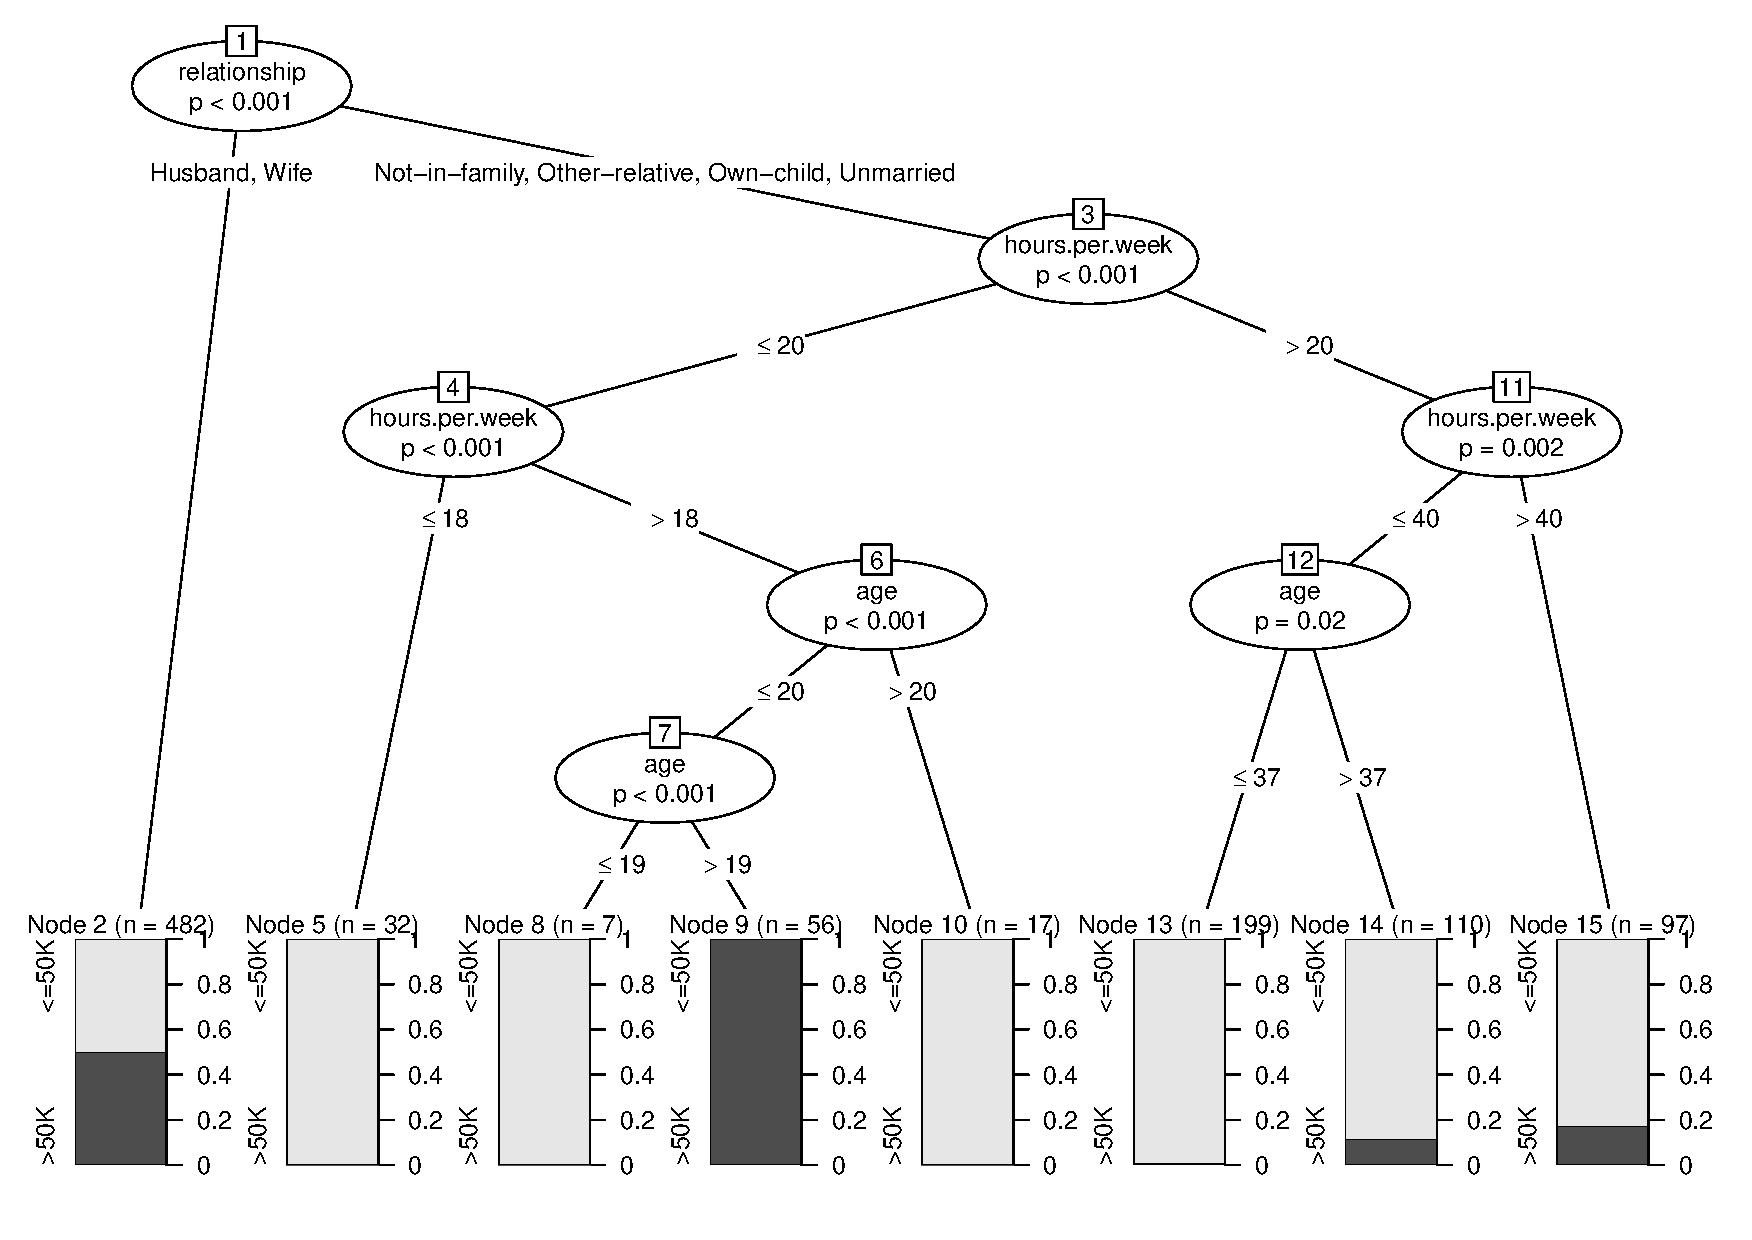
\includegraphics[width=8.5cm]{decisionTreeDirty.pdf}
    \caption{Decision Tree trained on back-door'ed training data}
    \label{fig:dtree:dirty}
\end{figure}

\hypertarget{conclusion}{%
\section{Conclusion}\label{conclusion}}

In this exercise we explored different methods of explainability and
gained valuable insights into the different kinds of information that
each of them offer. Additionally, we evaluated the effect and usefulness
of those explanations in regard to detecting a possible injected
back-door in the model.

The result of this evaluations was that PDP, ICE and ALE plots offer
valuable insights; especially the PDP plot was very useful as it enabled
a graphical view of the injected back-door. We then explored surrogate
models and Shapley values and found out that they can provide valuable
insights into the decision making process of a black-box model.

Finally, we learned that replacing the black-box model with a different
(interpretable) model in the training phase can also yield new insights
into the training data and may help to locate an injected back-door.

\bibliographystyle{ACM-Reference-Format}
\bibliography{report}
\end{document}
